\documentclass[a4paper,11pt]{article}
\usepackage[top=3cm, bottom=3cm, left=3cm , right=3cm]{geometry}
\usepackage[T1]{fontenc}
\usepackage[utf8]{inputenc}
\usepackage{lmodern}
\usepackage[francais]{babel}
\usepackage{authblk}
\usepackage{tabularx}
\usepackage{longtable}
\usepackage{array}
\usepackage{listings}
\usepackage{color}
\usepackage{float}
\usepackage{graphicx}


\begin{document}

\begin{titlepage}
  \newcommand{\HRule}{\rule{\linewidth}{0.5mm}} % Defines a new command for the horizontal lines, change thickness here

  \center % Center everything on the page
   
  %----------------------------------------------------------------------------------------
  %	HEADING SECTIONS
  %----------------------------------------------------------------------------------------

  \textsc{\LARGE INSA de Lyon}\\[1.5cm] % Name of your university/college
  \textsc{\Large DASI}\\[0.5cm] % Major heading such as course name
  \textsc{\large Collect'IF : partie 1}\\[0.5cm] % Minor heading such as course title

  %----------------------------------------------------------------------------------------
  %	TITLE SECTION
  %----------------------------------------------------------------------------------------

  \HRule \\[0.4cm]
  { \huge \bfseries Dossier d'analyse}\\[0.1cm] % Title of your document
  \HRule \\[1.5cm]
   
  %----------------------------------------------------------------------------------------
  %	AUTHOR SECTION
  %----------------------------------------------------------------------------------------

  % If you don't want a supervisor, uncomment the two lines below and remove the section above
  \Large \emph{Auteurs:}\\[1cm]
  \newcolumntype{R}{>{\raggedleft\arraybackslash}X}
  \newcolumntype{L}{>{\raggedright\arraybackslash}X}
  \begin{table}[h]
    \begin{center}
      \begin{tabularx}{10cm}{R L}
         Pierre-louis & \textsc{Lefebvre} \\
         Nicolas & \textsc{Six} \\[5cm]
      \end{tabularx}
    \end{center}
  \end{table}
  
  %----------------------------------------------------------------------------------------
  %	DATE SECTION
  %----------------------------------------------------------------------------------------

  {\large \today}\\[3cm] % Date, change the \today to a set date if you want to be precise

  %----------------------------------------------------------------------------------------
  %	LOGO SECTION
  %----------------------------------------------------------------------------------------

  %\includegraphics{Logo}\\[1cm] % Include a department/university logo - this will require the graphicx package
   
  %----------------------------------------------------------------------------------------

  \vfill % Fill the rest of the page with whitespace

\end{titlepage}
\tableofcontents
\pagebreak

%end header

\section{Modèle du domaine}

\begin{figure}[h]
  \begin{center}
    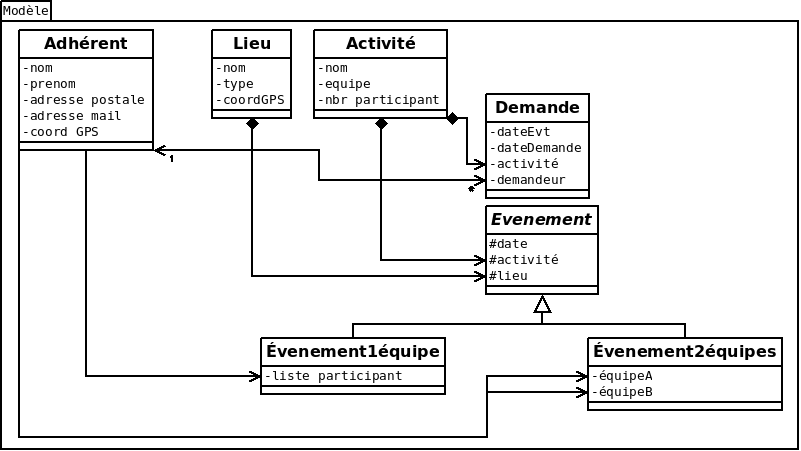
\includegraphics[width=15cm]{../modèle.png}
    \caption{Modèle du domaine}
  \end{center}
\end{figure}

\section{Description des services}

\paragraph{}
Afin d'assurer le bon fonctionnement de l'aplication nous avons dénombré un certain nombre de services nécéssaires à l'application. Ces services sont rassemblés ci-desous sous forme d'un tableau reprenant les éléments présent dans la JavaDoc.

\newcolumntype{P}[1]{>{\raggedright}p{#1}}

\begin{table}[H]
  \begin{center}
    \caption{ServicesMetier.java}
    \label{tab:ServicesMetier}
    \begin{longtable}{|P{7cm}|p{7cm}|}
      \hline
       void affecterLieuAEvenement(Lieu lieu, Evenement evenement) & Affecte un lieu a un evenement et envoye le mail correspondant \\ \hline
       List<Demande> afficherDemandesTrierParActiviteeDesc() & Renvoie la liste des demandes contenues dans la base de données, triée par nom d'activitee decroissant  \\ \hline
       List<Demande> afficherDemandesTrierParDateDescPourAdherent(Adherent adherent) & Renvoie la liste des demandes de l'adherent donnee en parametre, trier par ordre de date decroisante  \\ \hline
       void creerActivite(Activite activite) & Methode permettant d'ajouter une activité a la base  \\ \hline
       int creerAdherent(Adherent adherent) & Methode permettant d'ajouter un adherent a la base, seulement si celui-ci identifié par son adresse mail n'existe pas déjà dans la base de données, gère aussi l'envoi des mails d'infirmation ou de confirmation d'inscription  \\ \hline
       void creerDemande(Demande demande) & Ajoute a la base de données une demande  \\ \hline
       void creerEvenement(Evenement evenement) & Ajoute a la base de données un evenement  \\ \hline
       void creerLieu(Lieu lieu) & Methode permettant d'ajouter un lieu a la base  \\ \hline
<<<<<<< HEAD
       List<Activite> obtenirActivitees() & Renvoie la liste complète des activités presentes dans la base de données  \\ \hline
       List<Demande> obtenirDemandesTrierParActivitee() & Renvoie la liste des demandes contenues dans la base de données, triées par nom d'activité croissant  \\ \hline
       List<Demande> obtenirDemandesTrierParDatePourAdherent(Adherent adherent) & Renvoie la liste des demandes de l'adhérent donné en paramètre, trié par ordre de date croissante  \\ \hline
       List<Evenement> obtenirEvenementSansLieu() & Méthode renvoyant une liste de tous les événements affectés a aucun lieu  \\ \hline
       List<Lieu> obtenirLieux() & Renvoie la liste des Lieux contenus dans la base de donnée  \\ \hline
       Evenement rechercherEtCreerEvenement(Activite activite, java.util.Date date) & Renvoie l'evenement créé si la creation a eu lieu, null sinon  \\ \hline
       Activite trouverActivite(java.lang.String nom) & Renvoie l'activité corespondant au nom fourni  \\ \hline
       Adherent trouverAdherent(long id) & Renvoie l'adhérent corespondant a l'ID fourni  \\ \hline
       Adherent trouverAdherent(java.lang.String mail) & Renvoie l'adhérent corespondant au mail fourni  \\ \hline
       Evenement trouverEvenement(long id) & Renvoie l'événement corespondant a l'ID fourni  \\ \hline
       Lieu trouverLieu(long id) & Renvoie le lieu corespondant a l'ID fourni \\ \hline
=======
       List<Activite> obtenirActivitees() & Renvoie la liste complete des activitees presante dans la base de donnee  \\ \hline
       List<Demande> obtenirDemandesTrierParActivitee() & Renvoie la liste des demandes contenue dans la base de donnee, trier par nom d'activitee croissant  \\ \hline
       List<Demande> obtenirDemandesTrierParDatePourAdherent(Adherent adherent) & Renvoie la liste des demandes de l'adherent donnee en parametre, trier par ordre de date croisante  \\ \hline
       List<Evenement> obtenirEvenementSansLieu() & Methode renvoye une liste de tous les evenements affectes a aucun lieu  \\ \hline
       List<Lieu> obtenirLieux() & Renvoie la liste des Lieux contenue dans la base de donnee  \\ \hline
       Evenement rechercherEtCreerEvenement(Activite activite, java.util.Date date) & Renvoie l'evenement creer si la creation a eu lieu, null sinon  \\ \hline
       Activite trouverActivite(java.lang.String nom) & Renvoie l'activite corespondant au nom fournie  \\ \hline
       Adherent trouverAdherent(long id) & Renvoie l'adherent corespondant a l'ID fournie  \\ \hline
       Adherent trouverAdherent(String mail) & Renvoie l'adherent corespondant au mail fournie  \\ \hline
       Evenement trouverEvenement(long id) & Renvoie l'evenemnt corespondant a l'ID fournie  \\ \hline
       Lieu trouverLieu(long id) & Renvoie le lieu corespondant a l'ID fournie \\ \hline
>>>>>>> ef4bbbe04847a16217463b3dc9d3fabb29b3730e
    \end{longtable}
  \end{center}
\end{table}

\begin{table}[H]
  \caption{ServiceTechnique.java}
  \label{tab:ServiceTechnique}

  \begin{center}
    \begin{tabular}{|P{7cm}|p{7cm}|}
    \hline
       static void mailConfirmationInscriptionAdherent(Adherent adherent) & Affiche sur la console le mail que l'adhérent passé en paramètre recoit en cas de confirmation de son inscription \\ \hline
       static void mailConfirmationInscriptionResponsable(Adherent adherent) & Affiche sur la console le mail que le responsable recoit en cas de confirmation de l'inscription d'un adherent passe en paramètre \\ \hline
       static void mailEvenement(Evenement evenement) & Affiche sur la console le mail que le responsable envoie en cas de creation d'un evenement passe en paramètre \\ \hline
static void mailInfirmationInscriptionAdherent(Adherent adherent) & Affiche sur la console le mail que l'adhérent passé en paramètre recoit en cas d'infirmation de son inscription \\ \hline
static void mailInfirmationInscriptionResponsable(Adherent adherent) & Affiche sur la console le mail que le responsable recoit en cas d'infirmation de l'inscription d'un adhérent passe en paramètre \\ \hline
static void majCoordonnees(Adherent adherent) & Méthode de mise a jour de la latitude et longitude d'un Adhérent passé en paramètre \\ \hline
static void majCoordonnees(Lieu lieu) & Méthode de mise a jour de la latitude et longitude d'un Lieu passé en paramètre \\ \hline
    \end{tabular}
  \end{center}
\end{table}


\pagebreak
\section{Maquette des IHMs}

\subsection{IHM Utilisateur}

\subsubsection{Schéma général}

\paragraph{}
L'interface utilisateur est composée de deux vues distinctes: une vue de connexion et une d'utilisation. La première est déclinée en quatre variantes différentes en fonction des informations à afficher sur la page.

Les différents liens entre ces interfaces graphiques sont explicités sur la Figure~\ref{IHMs} qui représente les différents cas d'utilisation de la vue de connexion. Il est important de préciser que même avec l'affichage d'un message d'erreur ou de confirmation, la vue de connexion est toujours utilisable et se comporte comme une vue de connexion normale. De plus comme il le sera expliqué plus tard il est possible de revenir à la vue de connexion une fois sur la vue d'utilisation en utilisant le bouton "déconnexion".

\begin{figure}[H]
  \begin{center}
    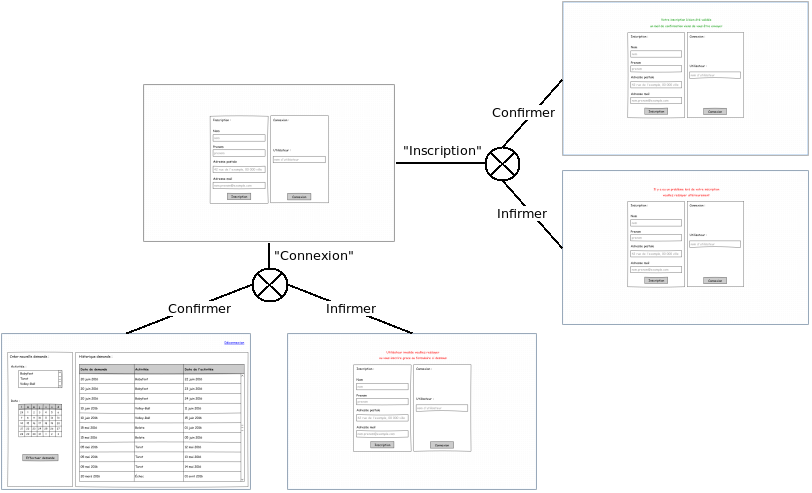
\includegraphics[width=15cm]{../../IHM/graphique_IHM.png}
    \caption{Mise en relation des IHMs}
    \label{IHMs}
  \end{center}
\end{figure}
\pagebreak
\subsubsection{IHM de connexion du client}

\paragraph{}
Cette IHM permet à l'utilisateur de se connecter à Collect'IF par simple saisie de sont adresse mail dans le menu de connection de la colonne de droite ou, dans le cas où celui-ci ne possède pas encore de compte, de s'en créer un grâce au menu d'inscription de la colonne de gauche.

\begin{figure}[H]
  \begin{center}
    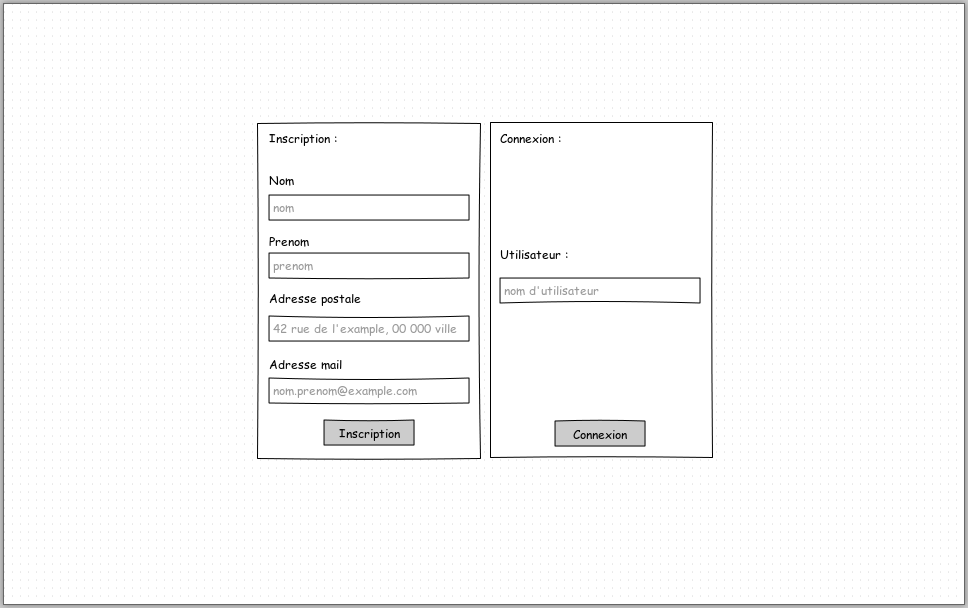
\includegraphics[width=15cm]{../../IHM/IHM_connection_utilisateur.png}
    \caption{IHM de connexion du client}
  \end{center}
\end{figure}

\newcolumntype{M}[1]{>{\centering}m{#1}}
\begin{table}[H]
  \begin{center}
    \begin{tabular}{|c|c|c|M{4cm}|m{4cm}|}
       \hline
       \textbf{Intention} & \textbf{Contrôle} & \textbf{Action} & \textbf{Réponse} & \textbf{Service }\\ 
       \hline
       Initialisation & - & - & - & - \\ 
       \hline
       Connexion & Bouton & Clic & Lien vers "IHM utilisateur" & trouverAdherent (String~mail)\\ 
       \hline
       Inscription & Bouton & Clic & Message sur la page courrante & creerAdherent (Adherent~adherent) \\ 
       \hline
    \end{tabular}
  \end{center}
\end{table}

\paragraph{}
Comme expliqué plus haut et illustré dans la Figure~\ref{IHMs}, en fontion de l'action effectuée ainsi que des données saisies, différents messages de confirmation ou d'erreur peuvent être affichés. Des illustrations de ces différents messages vous sont proposés ci-dessous.

\begin{figure}[H]
  \begin{center}
    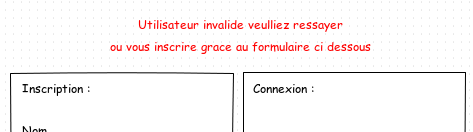
\includegraphics[width=15cm]{../../IHM/IHM_connection_utilisateur_erreur_co_z.png}
    \caption{IHM erreur de connexion du client}
  \end{center}
\end{figure}

\begin{figure}[H]
  \begin{center}
    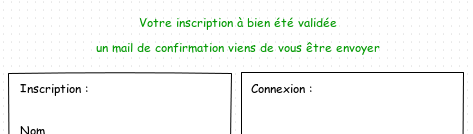
\includegraphics[width=15cm]{../../IHM/IHM_connection_utilisateur_conf_ins_z.png}
    \caption{IHM confirmation d'inscription}
  \end{center}
\end{figure}

\begin{figure}[H]
  \begin{center}
    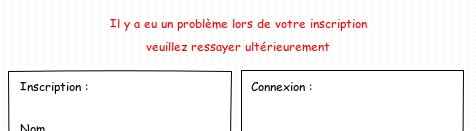
\includegraphics[width=15cm]{../../IHM/IHM_connection_utilisateur_erreur_ins_z.png}
    \caption{IHM erreur d'inscription}
  \end{center}
\end{figure}

\pagebreak
\subsubsection{IHM utilisateur}

\paragraph{}
L'IHM de l'utilisateur est décomposé en deux colonnes. La première sert à créer une nouvelle demande d'événement. Afin de l'aider dans cette tâche, l'utilisateur à accès à une liste des activités possibles dans laquelle il peut trouver facilement ce qu'il recherche en entrant la première lettre du nom de l'activié qu'il souhaite. De plus, graçe à une vue de type calendrier, il peut choisir le jour où il voudrait pratiquer cette activité.

La seconde colonne affiche l'historique des demandes de l'utilisateur comprenant la date de demande, le type d'activité demandé ainsi que la date choisie pour l'évènement, triées par date de demande.

Un bouton de déconnexion est aussi proposé à l'utilisateur ; ce lien lui permet de cloturer sa session et de revenir simplement sur la page de connexion.

\begin{figure}[H]
  \begin{center}
    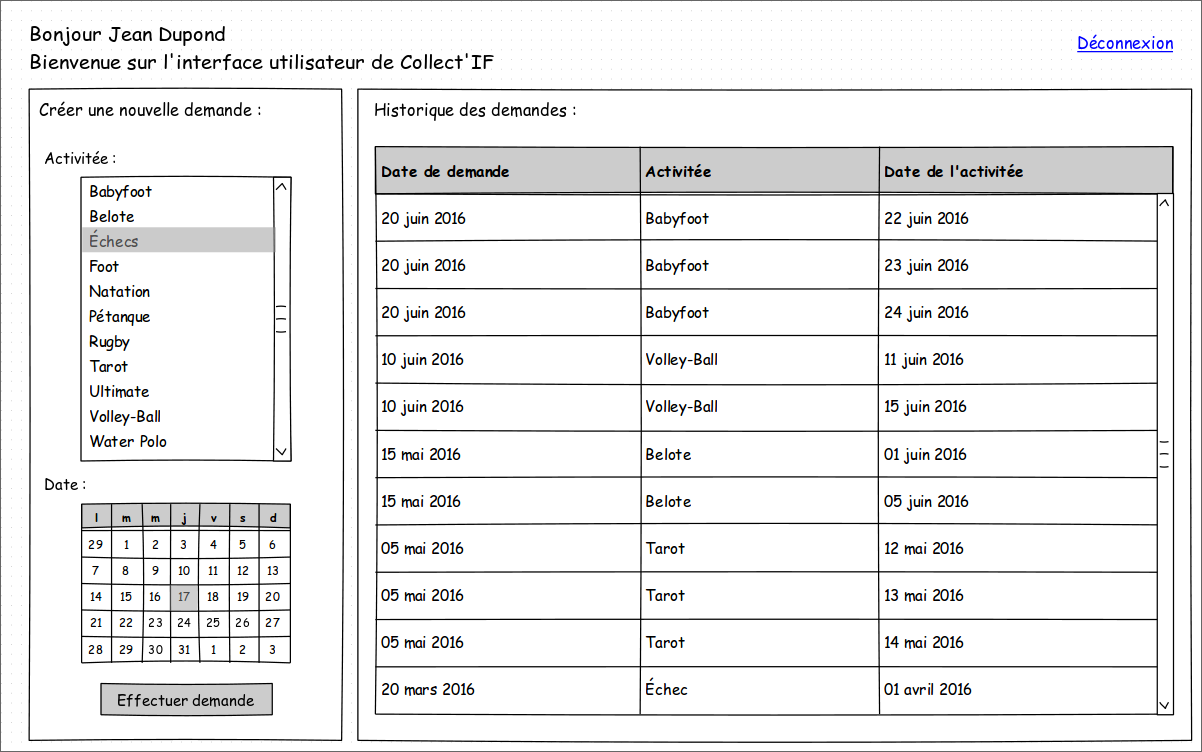
\includegraphics[width=15cm]{../../IHM/IHM_utilisateur.png}
    \caption{IHM utilisateur}
  \end{center}
\end{figure}

\begin{table}[H]
  \begin{center}
    \begin{tabular}{|M{2.5cm}|c|c|M{3cm}|m{5cm}|}
       \hline
       \textbf{Intention} & \textbf{Contrôle} & \textbf{Action} & \textbf{Réponse} & \textbf{Service} \\ 
       \hline
       Initialisation & - & - & - & afficherDemandesTrierParDate DescPourAdherent (Adherent~adherent) \\ 
       \hline
       Initialisation & - & - & - & obtenirActivitees() \\ 
       \hline
       Déconnexion & Bouton & Clic & Lien vers "IHM connexion" & - \\ 
       \hline
       Éffectuer une demande & Bouton & Clic & - & creerDemande (Demande~demande) \\ 
       \hline
    \end{tabular}
  \end{center}
\end{table}

\pagebreak
\subsection{IHM Administrateur}

\paragraph{}
L'IHM du responsable est composée de deux colonnes principales dont la première est remplie par une liste des évènements sans lieu, affichant la date et le type d'activité concerné. La seconde colonne est quant à elle destinée à afficher les détails de l'évènement sélectionné dans la liste de la première colonne au responsable afin de l'aider dans le choix du lieu pour l'événement. Cette vue est ainsi composée d'un rappel de la date et de l'activité concernée ainsi que d'une carte affichant les positions géographiques des logements des différents participants à l'événement. Cette carte affiche de plus les différents lieux qui peuvent être affectés pour l'évènement. Le lieu à affecter à l'évènement peut ensuite être choisi soit en selectionnant directement sur la carte soit en utilisant le menu déroulant en dessous, ce menu étant équipé d'un fonction de recherche permettant d'accéder rapidement à un lieu connu par le responsable.

L'IHM du responsable n'étant accesible que depuis un lieu particulier il n'est pas nécessaire d'avoir une interface de connexion et de déconnexion.

\begin{figure}[H]
  \begin{center}
    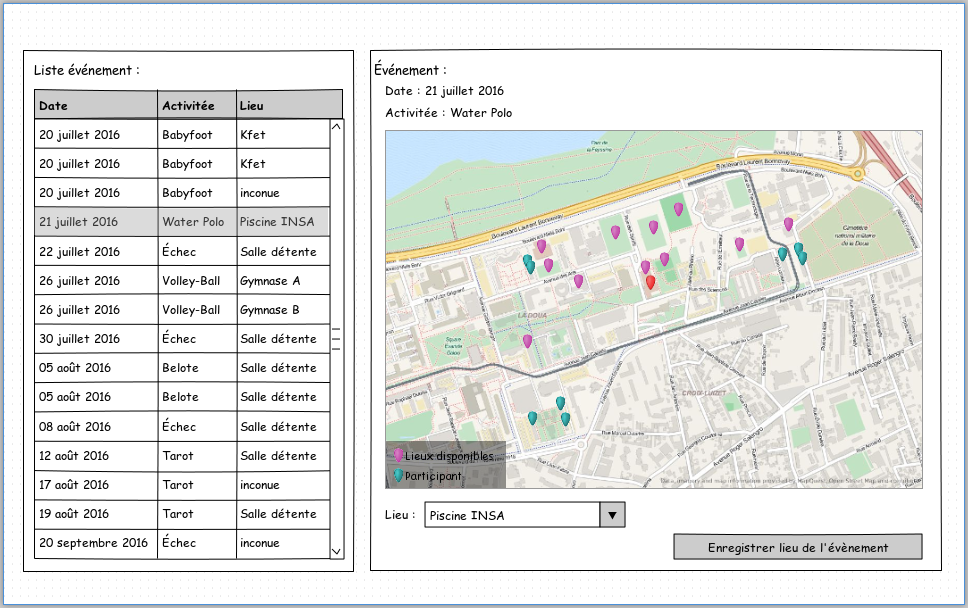
\includegraphics[width=15cm]{../../IHM/IHM_responsable.png}
    \caption{IHM Administrateur}
  \end{center}
\end{figure}

\begin{table}[H]
  \begin{center}
    \begin{tabular}{|m{4cm}|m{10cm}|}
       \hline
       \textbf{Bouton} & \textbf{Action} \\
       \hline
       Enregistrer lieu de l'évènement & L'évènement courrant est modifier dans la base de donnée de façons à ce que le lieu sélectionné lui soit affecté.   \\
       \hline
    \end{tabular}
  \end{center}
\end{table}


\end{document}
